%! Author = abenjeddou
%! Date = 29/05/2026

% Preamble
\section{Introduction}
This chapter was written with the intention of providing a clear overview of the host organisation, the different departments and the context of our project.
To do this, we will undertake an analysis of the current situation in order to clearly define the solution we are considering.
\section{The host organisation}
In this section we will present the host organisation.
\subsection{Orange group}
Orange is one of the world's leading telecommunications operators, with sales of 42.3 billion euros in 2020 and 142,000 employees worldwide as of December 31, 2020, including 82,000 in France. The group had a total of 259 million customers worldwide as of December 31, 2020, including 214 million mobile customers and 22 million fixed broadband customers. The group is present in 26 countries. Orange is also a major provider of global IT and telecommunications services for multinational companies, under the Orange Business Services brand. In December 2019, the group presented its new "Engage 2025" strategic plan, which, guided by social and environmental responsibility, aims to reinvent its operator model. While accelerating in growth areas and placing data and AI at the heart of its innovation model, the group will be an attractive and responsible employer, suitable for emerging professions.
\subsection{Sofrecom Tunisie}
A subsidiary of the Orange Group, Sofrecom advises, guides and supports the development and digital transformation of the main telecommunications players (operators, governments and international institutions).

\subsection{Departments of sofrecom}
The software development department brings together talented and experienced developers who are responsible for designing and implementing state-of-the-art software. Java backend developers like myself work within this department to create high-performance and scalable applications, using the best development practices and the latest technologies.

The software architecture department plays a vital role in the design and planning of software systems.
Sofrecom Tunisia's software architects work closely with developers to define the overall architecture of applications, ensure their consistency and scalability, and oversee their implementation.

The Information Systems Security Department focuses on protecting applications and data from potential threats.
We, the developers, collaborate with security experts to implement strong authentication and authorization mechanisms, as well as secure coding practices.

\section{Project's context}

In the era of massive data proliferation, real-time data processing
constitutes a major challenge.
The ability to react instantly to events requires
the implementation of a robust and efficient system, capable of meeting customer requirements by
guaranteeing real-time responsiveness.
It is with this in mind that we are exploring the use of a framework for processing
massive data streams, specifically Apache Flink~\cite{FLINK}.
This choice will allow us to optimize
our data processing workflow in order to effectively meet our
specific needs.
This project is called \("\)Levee Fair Use\("\) or LFU in short.
It is a project that aims to set up a real-time data processing system for push notifications that allow users to know hen they reached their threshold of data consumption.

\subsection{Study of the existing method}
Currently, the message processing for our notifications is divided into two distinct steps.

First, as illustrated in Figure 1.1, a Java daemon runs continuously to
retrieve messages from RabbitMQ \cite{RBMQ}, performs the necessary transformations, and then
finally stores them in the database.
\begin{center}
    \centering
    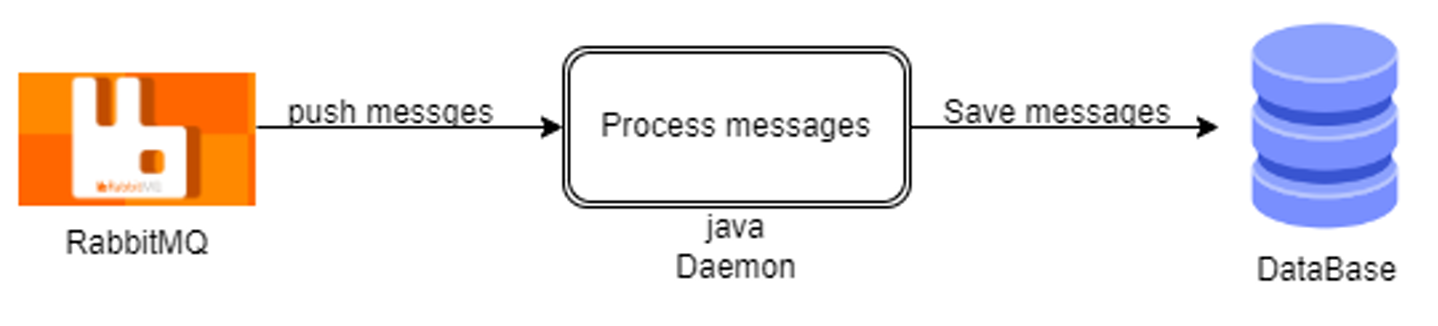
\includegraphics[width=1\textwidth,height=4.5cm]{img/demon java}
    \captionof{figure}{Daemon java}
\end{center}
Next, as shown in Figure 1.2, a batch process is scheduled to run twice a day to process and send the messages that have been previously stored to the Erable API, which then notifies the clients.
\begin{center}
    \centering
    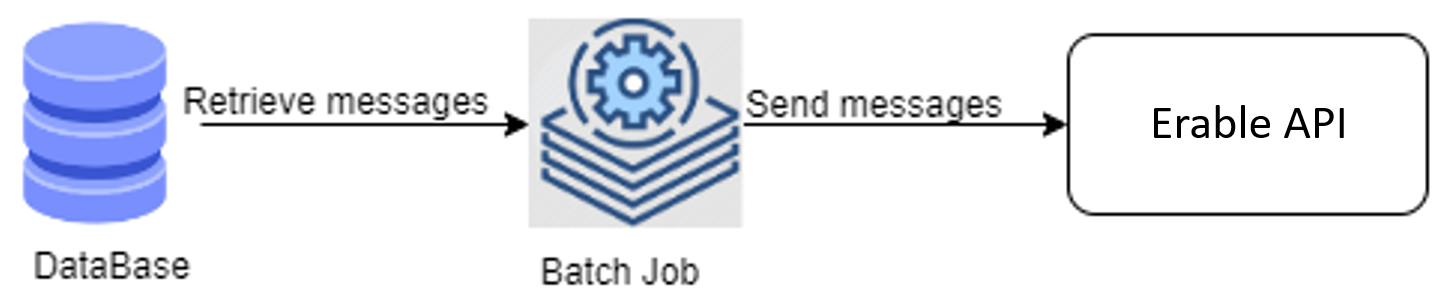
\includegraphics[width=1\textwidth,height=4cm]{img/batch job}
    \captionof{figure}{Batch job}
\end{center}
\subsection{Critique of the existing method}
After studying how the current solution works, we identified the following shortcomings:
\begin{itemize}
    \item[-] \textbf{Notification delay:} Notifications are generated with a delay due to the periodic execution of batch processes.
    \item[-] \textbf{Inability to handle variable workloads:} Scalability is too difficult and costly to implement during data spikes, causing significant delays.
    \item[-] \textbf{Late anomaly detection:} This leads to a delay in responding to problems.
    \item[-] \textbf{Architecture complexity:} Managing and scheduling batch process launches.
    \item[-] \textbf{Resource waste:} Batch processes are triggered even when there is no data to process, resulting in a waste of resources that could have been avoided.
    \item[-] \textbf{Maintenance:} Maintaining an architecture divided into two parts could require more effort and resources.
\end{itemize}

\subsection{Proposed solution}
The objective of our project is to set up a system for processing massive data streams in real time.
This system will connect directly to RabbitMQ as a data source, will process events as they arrive, then send them to Erable API. The latter will in turn be responsible for distributing them to customers, thus providing immediate responsiveness and improving the customer experience by guaranteeing instant receipt of notifications.

In case of an increase in workload, we will be able to automatically launch processing instances on the fly, without requiring manual intervention.
Furthermore, the detection of issues will be accelerated, allowing rapid action.

It is essential to integrate a monitoring and supervision block to efficiently exploit the logs and metrics from our system.
This will facilitate the investigation process in case of any problems.

We will also integrate an AI module that allows us to predict if the user is going to exceed their data quota based on their consumption patterns.
\begin{center}
    \centering
    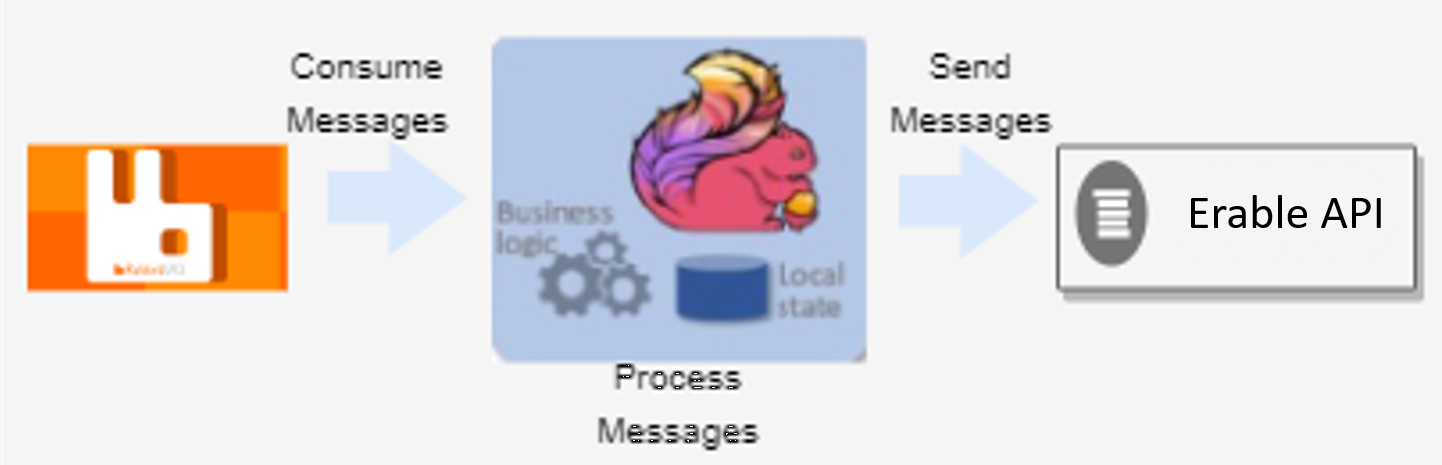
\includegraphics[width=1\textwidth,height=5cm]{img/Solution}
    \captionof{figure}{Targeted solution}
\end{center}
\section{Scrum Methodology}
This section is dedicated to the explanation of the agile methodology utilized to
construct the solution.

\subsection{Scrum definition}
Scrum methodology is one of the most widely used agile development methodolo
gies out there.
It is an adaptable and flexible framework mostly, but not only, used
for software development.
Scrum relies on its incremental and iterative processes
to best deliver value to the customer all along the project development [2].
Such methodology contains a set of principles that need to be respected and followed during the development process.
In the following sections, we will explain the Scrum roles and procedure.
\subsection{Scrum roles}
Scrum methodology requires a team of: a scrum master, a product owner, and a team
of developers.
\begin{itemize}
    \item \textbf{The scrum master:} is the team leader.
    She instructs the team on how to
    follow the methodology’s rules.
    If necessary, she also coaches and mentors the
    team.
    \item[-] \textbf{The product owner:} his role is to represent the stakeholders and customers translating the envisioned product to the team.
    \item[-] \textbf {Development team:} which corresponds to a group of professionals who possess the necessary technical skills to efficiently develop the product following
    its different increments
\end{itemize}

\subsection{Scrum process}
When following the Scrum methodology, the project gets divided into many iterations called \("\)sprints\("\).
But firstly, before defining the sprints, the product owner is required to write the Product Backlog, which is a document that has all the functionalities determined by the stakeholders. Afterwards, the team takes care of creating both the user stories and sprint backlog. Finally, the development team gets to work on the various sprints, which last around two to four weeks and during which the team concentrates on analyzing and creating the sprint. The scrum master ensures that her team respects the scrum methodology throughout the entire process. At the conclusion of the expected time frame, a meeting is held where the team delivers their finished work, different functionalities from the product backlog are selected and the previous procedures are repeated in preparation for the following sprint.

Figure 1.4 below describes the Scrum process
\begin{center}
    \centering
    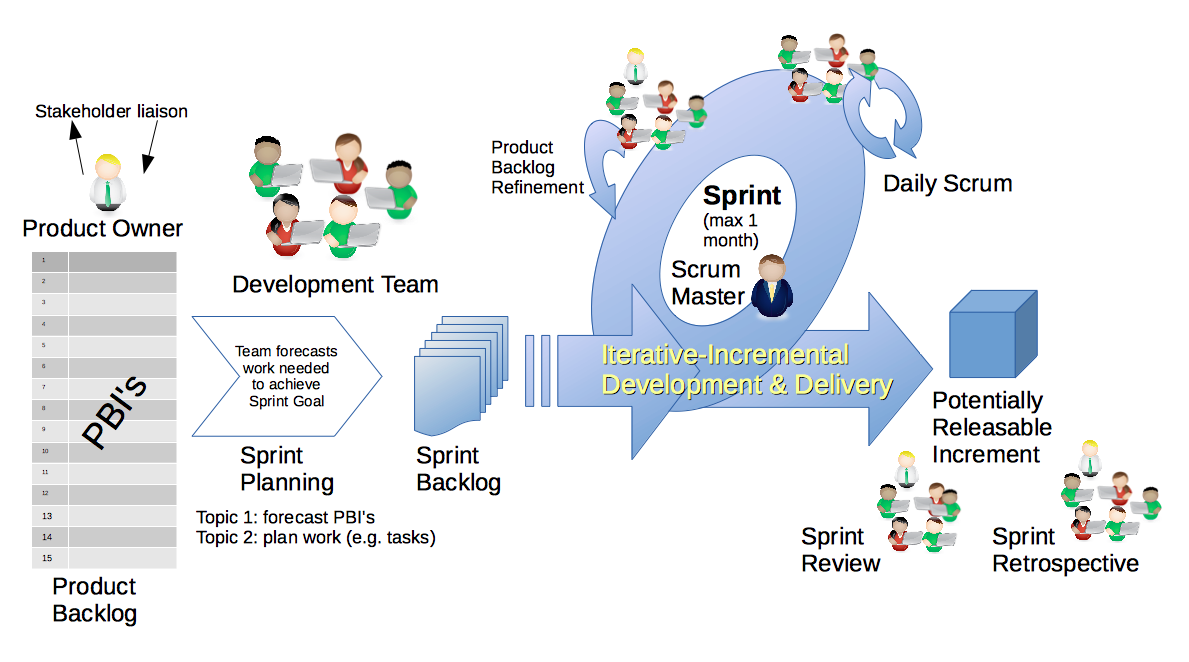
\includegraphics[width=1\textwidth,height=8cm]{img/Scrum_Framework}
    \captionof{figure}{Targeted solution~\cite{scrum}}
\end{center}



\section*{Conclusion}
In the first chapter, we started with the presentation of the general idea of our
project and the host establishment.
We later analyzed the existing method used in our current process.
We criticised the current method by listing its different shortcomings, and then we proposed a solution that will allow us to overcome them.
Finally, we discussed the agile methodology that was applied to this project.
The software requirements and requirement analysis for our project will be examined in the next chapter.